\let\conjugatet\overline
\chapter{Synchronisation}
\todo{Signalmodell, Annahmen, Einflüsse, usw}
\section{Zeit Synchronisation}
Eine geeignete Zeitsynchonisation muss sowohl eine grobe Synchronisation des OFDM Frames als auch eine feine Synchonisation der einzelnen OFDM Symbole sicherstellen. \\

Der Beginn eines jeden Frames $ k $ wird durch das Nullsymbol $z_{0,k}$ markiert. Wegen $S(t) = 0$ für $t \in [0, T_{NULL}]$ stellt es eine zuverlässige Möglichkeit dar den Anfang eines Frames über eine Energiemessung zu detektieren.
\todo{Formel Energie aber Intervall kürzer als T NULL}

\begin{equation}
E[i] = \sum \limits_{j=i}^{T_G}|x[j]|^2
\label{eq:energy}
\end{equation}

Nachdem der Anfang eines Frames detektiert wurde, muss im Folgenden der Beginn jedes OFDM Symbols $z_{l,k}$ ($l \in [1, 76]$) festgelegt werden. Diese feine Zeitsynchronisation erfordert keine sehr hohe Genauigkeit, da jedem Symbol ein Cyclic Prefix der Dauer $T_G = 246 \mu s $ vorgeschoben ist, dessen Inhalt dem Ende des eigentlichen Symbols entspricht. Dadurch ergibt sich ein Zeitbereich von  $T_D \in [0,T_G]$ in dem das Symbol fehlerfrei gesetzt werden kann, also das gesetzte Symbolfenster nicht in das vorhergehende oder nachfolgende Symbol hereinragt.

% cyclic prefix figure
\begin{figure}
\begin{center}
\begin{tikzpicture}
\newcommand{\ursprung}{(0,0)}
\node[] at \ursprung (null) {}; 
\draw [thick, rounded corners = 6pt] 
    (null) -- ++(0,0.5) -- ++(0,0.5) -- ++(8,0) -- ++(0,-1) -- ++(-8,0) -- ++(0,0.5);
\draw [dashed]
    (null)+(2,0) -- ++(2,1);
\draw [dashed]
    (null)+(6,0) -- ++(6,1);
\node[] at (1,1.5) (guard) {$T_G$};
\draw [<-] (0,1.5) -- (guard.west);
\draw [->] (guard.east) -- (2,1.5);
\node[] at (5,1.5) (symbol) {$T_S$};
\draw [<-] (symbol)+(-3,0) -- (symbol.west);
\draw [->] (symbol) -- (8,1.5);
\node[] at (0.75,-0.5) (delay) {$T_D$};
\draw [<-] (delay)+(-0.75,0) -- (delay.west);
\draw [->] (delay) -- (1.5,-0.5);
%Beschriftung
\node[] at (1,0.5) (cp) {CP};
\node[] at (7,0.5) (cp) {CP Quelle};
%Vorgängersymbol
\draw [thick, rounded corners = 6pt]
    (-1.5,0) -- ++(1.5,0) -- ++(0,1) -- ++(-1, 0);
\draw [decorate,decoration={snake, amplitude=.4mm}] (-1.5,0) -- (-1,1);
%Nachfolgersymbol
\draw [thick, rounded corners = 6pt]
    (9,0) -- ++(-1,0) -- ++(0,1) -- ++(1.5, 0);
\draw [decorate,decoration={snake, amplitude=.4mm}] (9,0) -- ++(0.5,1);
%gesetztes Symbolfenster
\draw[-,decorate,decoration=brace] 
    (7.5,-0.2) -- (1.5,-0.2) node [midway, yshift=-0.3cm]{};
\node[] at (4.5,-0.6) {gesetztes Symbolfenster für $z_{l,k}$};
\end{tikzpicture}
\end{center}
\caption{OFDM Symbol und Cyclic Prefix}
\label{chart:cp}
\end{figure}

Um \ac{ISI} zu minimieren ist der theoretisch optimale Abtastzeitpunkt genau am Ende des Cyclic Prefix zu wählen. Eine komplette \ac{ISI} Unterdrückung ist wegen $T_G < \tau_{max}$ mit einer maximalen Echo Verzögerung von $\tau_{max} = 300 \mu s$ \todo{cite} nicht möglich. Jedoch wird die \ac{ISI} zu einem Minimum reduziert, wenn ein maximal später Startpunkt gewählt wird, da dadurch die Interferenzzeit $\tau_{max} - T_G$ (bei $\tau_{max} < T_G+T_S$) minimiert wird.

\todo{Bild mit Symbol und evt Frame, wo Zeitreferenz markiert ist, auf dem dann die Formeln/Delays basieren können}

Um den exakten Anfang eines Symbols zu bestimmen, wird die zyklische Wiederholung des Symbolanteils im Cyclic Prefix genutzt. Durch eine Korrelation des abgetasteten Empfangssignal $x[i]$ mit einer um $T_S$ verzögerten Version desselben Signals $x[i+T_S]$ über das Intervall $[i, i+T_G]$ kann der Anfang des Cyclic Prefix über einen Peak der Korrelation identifiziert werden.

\todo{klären, wann $T_G$ Zeit und wann samples angibt, bzw anderes symbol verwenden}
%einfache correlation
\begin{equation}
y[i] = \sum \limits_{j=i}^{T_G}r[j] \conjugatet{r[j+T_S]}, \ \ y[i] \in \mathbb{C}
\label{eq:corr_einfach}
\end{equation}

Unter Berücksichtigung von additivem weißen Rauschen r[i]=x[i]+n[i] mit $N[i] \sim \mathcal{N}(\mu,\,\sigma^{2})$ ergibt sich

\begin{equation}
    \begin{aligned}
y[i] &= \sum \limits_{j=i}^{T_G}(x[j]+N[j]) \conjugatet{(x[j+T_S]+N[j])} \\
&= \sum \limits_{j=i}^{T_G}x[j] \conjugatet{x[j+T_S]} + \sum \limits_{j=i}^{T_G}x[j] \conjugatet{n[j+T_S]} + \sum \limits_{j=i}^{T_G}n[j] \conjugatet{x[j+T_S]} + \sum \limits_{j=i}^{T_G}n[j] \conjugatet{n[j+T_S]} \\
&= P T_G + 2(P \sigma^2) + \sigma^4 \approx P T_G + 2(P \sigma^2)
    \end{aligned}
\end{equation}

und damit ein SNR des Korrelationssignals von
\begin{equation}
SNR = \frac{P_x}{P_n} = \frac{P T_G}{2 P \sigma^2} = \frac{T_G}{2 \sigma^2}
\end{equation}

Durch eine Mittelung über $T_G * Samplerate = 504$ Samples ist das SNR somit ausreichend groß um eine entprechend genaue Peakdetektion durchführen zu können.

\begin{figure}[ht]
\centering
  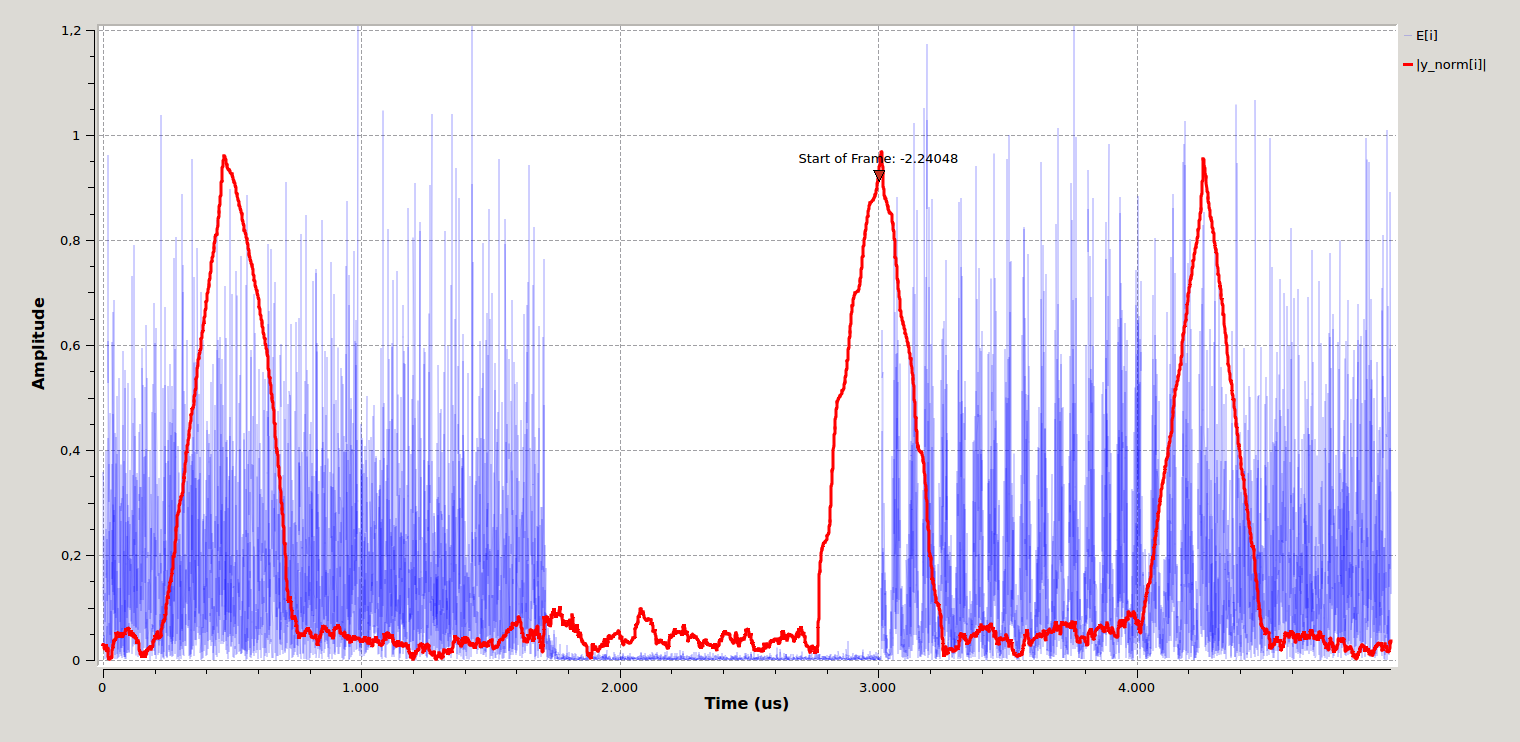
\includegraphics[width=0.8\textwidth]{figures/delayed_correlation_abs_and_energy.png}
	\caption{Korrelation des Cyclic Prefix}
	\label{fig:corr}
\end{figure}

Die Korrelation ist dabei auf die Energieanteile des Cyclic Prefixes und dessen Quelle nach $T_S$ normiert, sodass das Ergebnis unabhängig von der Empfangsleisung bleibt, die durch Empfangsqualität und verwendeter Hardware stark variieren kann.

\begin{equation}
    y_{norm}[i] = \frac{\sum \limits_{j=i}^{T_G}x[j] \conjugatet{x[j+T_S]}}{\sqrt{\sum \limits_{j=i}^{T_G}|x[j]|^2 \sum \limits_{j=i}^{T_G}|x[j+T_S]|^2}} = \frac{\sum \limits_{j=i}^{T_G}x[j]     \conjugatet{x[j+T_S]}}{\sqrt{E[i]E[i+T_S]}}
    \label{eq:norm_corr}
\end{equation}

In Abbildung~\ref{fig:corr} ist zu erkennen, dass die Flanken der Korrelation linear ansteigen. Die Breite einer Flanke entspricht $T_G$, also gerade dem Entscheidungsbereich für $T_D$. Durch die Linearität der Flanke und der Normierung, kann der relative Abtastzeitpunkt innerhalb des Cyclic Prefix über einen Schwellwert eingestellt werden. Der tatsächliche Abtastzeitpunkt wird anschließend mit einer Verzögerung von $T_G$ gestetzt. In der Implementierung von Abbildung~\ref{fig:corr} wurde ein Schwellwert von $0,85$ eingestellt, der sich als guter Kompromiss zwischen \ac{ISI} Unterdrückung und einem Sicherheitsabstand zu $T_D > T_G$ herausgestellt hat. Man beachte, dass $T_D > T_G$ dazu führt, dass Samples vom nachfolgenden Symbol im gesetzen Symbolfenster liegen was zum Empfang von falscher Information führt. Dieser Fall entspricht einer fehlerhaften Zeitsynchronisation.

\subsubsection{Implementierung}
Um eine mehrfache Berechnung von Gleichung~\ref{eq:energy} für die Energiemessung (Gl.~\ref{eq:energy}) sowie die normierte Korrelation (Gl.~\ref{eq:norm_corr}) zu vermeiden, wurde die feine und grobe Zeitsynchronisation in einer gemeinsamen Klasse implementiert.

\begin{figure}
\begin{center}
\begin{tikzpicture}[node distance = 2cm, auto]
% Define block styles
\tikzstyle{decision} = [diamond, draw, fill=cyan!30, 
    text width=4.5em, text badly centered, node distance=3cm, inner sep=0pt]
\tikzstyle{start} = [rectangle, draw, fill=cyan!30, 
    text width=5em, text centered, rounded corners, minimum height=4em]
\tikzstyle{output} = [trapezium, draw, fill=cyan!30, 
    text width=4em, text centered, minimum height=4em, trapezium right angle=110, trapezium left angle=70]
\tikzstyle{block} = [rectangle, draw, fill=cyan!30, 
    text width=5em, text centered, minimum height=4em]
\tikzstyle{line} = [draw, -latex']
\tikzstyle{cloud} = [draw, ellipse,fill=red!20, node distance=3cm,
    minimum height=2em]
    % Place nodes
    \node [start] (init) {Start};
    \node [decision, below of=init] (null) {NULL erwartet?};
    \node [block, below of=null, node distance=3cm] (corr) {gleitende Korrelation};
    \node [decision, below of=corr, node distance=3cm] (peak) {Peak?};
    \node [block, below of=peak, node distance=2.5cm] (energy) {Energie- messung};
    \node [decision, below of=energy] (first) {Symbol $z_{1,k}$?};
    \node [output, below of=first, node distance=3cm] (tag) {Start des Frames in $T_G$};
    \node [block, right of=null, node distance=4.5cm] (skip) {überspringe $T_S$};
    \node [block, below of=skip, node distance=3cm] (corr2) {einmalige Korrelation};
    \node [decision, below of=corr2] (peak?2) {Peak?};
    \node [above of=null, node distance=2cm] (backtonull){};
    \node [output, below of=peak?2, node distance=3cm] (lost track){nicht mehr in Sync};
    
    \path [line] (init) -- (null);
    \path [line] (null) -- node {ja} (corr);
    \path [line] (null) -- node {nein} (skip);
    \path [line] (corr) -- (peak);
    \path [line] (peak) -- node {ja} (energy);
    \path [line] (energy) -- (first);
    \path [line] (first) -- node {ja} (tag);
    \path [line] (peak) -- node {nein} ++(2.5cm,0);
    \path [line] (first) -- node {nein} ++(2.5cm,0) |- (corr);
    \path [line] (skip) -- (corr2);
    \path [line] (corr2) -- (peak?2);
    \path [line] (peak?2.south) -- node {nein} (lost track);
    \path [line] (peak?2.east) -- node{ja}++(1cm,0) -- ++(0,8cm) -- ++(-6.5,0);
    \path [line] (tag) -- node{}++(0,-1cm) -- node {} ++(-2.5cm,0) -- node{}++(0,17.5cm) -- ++(2.5cm,0);
    \path [line] (lost track.south) -- ++(0,-1cm) -- ++(-2,0);
\end{tikzpicture}
\end{center}
\caption{Programmablaufplan der Zeitsynchronisation}
\label{chart:zeitsync}
\end{figure}

Abbildung~\ref{chart:zeitsync} zeigt den Programmablaufplan der Zeitsynchronisation. Er ist aufgeteilt in die beiden Zweige "Suche Frame Start" und "Kontrolle". Der Zweig "Suche Frame Start" kommt bei einem der folgenden Fälle zum Einsatz:
\begin{itemize}
\item Die Synchronisation wird initial gestartet.
\item Das Programm ist nicht mehr in Synchronisation.
\item Das Ende eines Frames wurde erreicht.
\end{itemize}
Alle diese Situationen haben gemeinsam, dass im Folgenden nach dem Peak des Symbols $z_1,k$ (erstes Symobl nach dem Nullsymbol) gesucht wird. Es wird iterativ für jedes Sample des Zeitsignals $x[i]$ eine Korrelation $y[i]$ nach Gl.~\ref{eq:norm_corr} durchgeführt. Dadurch können (analog zu Abb.~\ref{fig:corr}) Korrelationspeaks detektiert werden die jeweils dem Start eines Symbols entsprechen. Durch die Energiemessung das Symbols $z_{1,k}$ von den restlichen Symbolen $z_{l,k},$ mit  $l \in [2,76]$ unterschieden werden.

Die Komplexität der Korrelationsoperation kann drastisch reduziert werden, indem die Summe, die laut Gl.~\ref{eq:corr_einfach} in jedem Schritt $T_G = 504$ Additionen durchführt, durch eine gleitende Summe ersetzt wird.
%gleitende Summe
\begin{equation}
    y[i+1] = y[i] - r[i] \conjugatet{r[i+T_S]} + r[i+T_G] \conjugatet{r[i+T_G+T_S]}
    \label{eq:moving_sum}
\end{equation}
Dabei ist zu beachten, dass natürlich $y[i=0]$ komplett berechnet werden muss. Um einen das Ergebnis verfälschenden Drift von $y[i]$ zu vermeiden, wird die Summe außerdem alle $i=100000$ Samples neu berechnet.

Wenn der Anfang von $z_{1,k}$ gefunden und festgelegt wurde, stehen auch die Anfänge aller anderen Symbole des Frames fest, da sie mit dem festen und bekannten Abstand von $T_G+T_S$ direkt aufeinanderfolgen. Der Zweig "Kontrolle" springt daher nur noch vom Start eines Symbols $x[i]$ zum Nächsten $x[i+T_G+T_S]$ und berechnet an dieser Stelle einmalig die Korrelation $y[i+T_G+T_S]$. Liegt $y[i+T_G+T_S]$ über einem Schwellwert, wurde das Sample als Anfang des nächsten Symbols bestätigt und die Kontrollschleife iteriert zum nächsten Symbol. Falls an einem erwarteten Symbolanfang der Schwellwert der Korrelation unterschritten wird, wechselt das Programm in den Zweig "Suche Frame Start".

Da die Symboldauer genau bekannt ist, mag eine Kontrolle von jedem einzelnen Symbol zunächst überflüssig erscheinen. Der Aufwand wird jedoch gerechtfertigt um Störeffekte wie einen Clockdrift rechtzeitig erkennen und korrigieren zu können bevor dieser zu einem Verlust der Synchronisation und damit zu Datenverlusten führen kann.
Ein beispielhafter Clockdrift von 50 ppm kann im rauschfreien Fall zu einem maximalen Phasenfehler von
\begin{equation}
\begin{aligned}
    \Delta\varphi_{max} = 2 \pi f_{max} \Delta t &= 2 \pi \frac{B}{2} Clockdrift (T_G+T_S) \\
    &=  2 \pi \frac{1536 Hz}{2} 50ppm 1246\mu s \\
    &= 0,3 rad = \ang{17,2}
    \end{aligned}
    \label{eq:clockdrift}
\end{equation}
führen. Rechnung~\ref{eq:clockdrift} zeigt, dass eine feine Zeitsynchronisation zu jedem Framebeginn zu wenig ist, da sich der Phasenfehler bei 76 Symbolen pro Frame aufsummiert und damit die Entscheidungsgrenzen einer QPSK Demodulation überschreitet. Damit ist der Zweig "Kontrolle" gerechtfertigt.


%%%%%%%%%%%%%%%%%%%%%%%%%%%%%%%%%%%%%%%%%%%%%%%%%%%%%%%%%%%%%%%%%%%%%%%%%%%%%%%%%%%%%%%%%%%%%%%%%%%
\section{Frequenz Synchronisation}
Die Messung und Korrektur eines Frequenzoffsets ist der nächste Schritt der Synchronisationskette. Sie spielt in OFDM Systemen eine besonders wichtige Rolle, da ein Frequenzoffset die Orthogonalität zwischen den Unterträgern zerstört und somit zu \ac{ICI} führt.

\subsection{Feine Frequenz-Schätzung}
Für die Messung des Frequenzoffsets kann wieder auf die Korrelaton aus Gl.~\ref{eq:corr_einfach} zurückgegriffen werden. Ein Frequenzoffset lässt sich hier als konstante Änderung der Phase über der Zeit $T_S$ messen, da die Phase von Cyclic Prefix und dessen Wiederholung ohne Frequenzoffset gleich sind. 
\begin{equation}
f_{off}[i] = \frac{arg(y[i])}{T_S}
\label{eq:fine_frequency_estimation}
\end{equation}
Ein zusätzliches \ac{AWGN} ändert die Phase jedes einzelnen Samples. Wegen der Mittelwertfreiheit von \ac{AWGN} kann die Varianz des gemessenen Frequenzoffsets durch eine Mittelung reduziert werden.
\todo{Rechnung zu Varianz bei Mittelung (Gleichverteilung mit unabh. ZVs als Ausgangspunk}
Durch das Korrelationsintervall von $T_G = 504$ Samples wird solche eine Mittelung durchgeführt was die relativ kleine Varianz der Frequenzoffsetmessung in Abb.~\ref{plot:varianz_freq_offset} bestätigt.
\todo{Wie korrigieren reinbringen}
\begin{center}
\todo{Werte noch nicht richtig, es muss ein rauschfreies sendesignal verwendet werden!}
\begin{tikzpicture}
\begin{axis}[
title=Varianz der feinen Frequenzoffsetmessung,
xlabel={$SNR \ [dB]$},
ylabel={$E((\hat{f} - f_{off})^2) \ [Hz]$},
grid=both,
]
\addplot [blue, mark=diamond*]table {data/171017_frequency_offset_variance_over_SNR.dat};
\end{axis}
\label{plot:varianz_freq_offset}
\end{tikzpicture}
\end{center}

Durch die aktive Mittelung über N Symbole wird eine weitere Senkung der Varianz um Faktor N erreicht. Pro Symbol wird genau eine Korrelation berechnet, also ergibt sich ein Mittelungsfenster der Dauer $N (T_G + T_S)$. Ein zu langes Mittelungsfenster führt zu einer Trägheit der Frequenzmessung und damit auch zu einer Zeitverzögerung in der Frequenzkorrektur, was bei schnellen Frequenzänderungen zu Synchronistaionsverlusten führen kann. Vor allem bei mobilen \ac{DAB} Empfängern wird dieser Fall aufgrund der Dopplerverschiebung relevant. Aus diesem Grund wird für die obere Grenze der Mittelung die Bedingung gestellt, dass bei einer maximalen, konstanten Beschleunigung $a$ der durch die Mittelung verursachte Messfehler $f_M$ unter der $3\sigma$ Grenze liegt.
\begin{equation}
f_M \overset{!}{<} \frac{3\sigma(SNR)}{\sqrt{N}}
\label{eq:3sigma_grenze}
\end{equation}
Mit $a=50m/s^2$ und einer Trägerfrequenz von $f_T = 200 MHz$ ist
\begin{equation}
\frac{df}{dt} = f_T * \frac{a}{c} = 33,3 Hz/s
\end{equation}
und damit
\begin{equation}
\begin{aligned}
f_M &= \frac{1}{N} \sum \limits_{i=0}^{N-1} i \frac{df}{dt} (T_G+T_S) \\
&= \frac{1}{N} \frac{df}{dt} (T_G+T_S) \left(\frac{N^2 + N}{2} - N\right) \ \ {\overset{N\text{groß}}{\approx}} \ \  \frac{df}{dt} (T_G+T_S) N
\end{aligned}
\label{eq:mittelung_fehler}
\end{equation}
Aus \ref{eq:3sigma_grenze} und \ref{eq:mittelung_fehler} ergibt sich eine rauschabhängige Obergrenze für das Mittelungsintervall.
\begin{equation}
N \overset{!}{<} \left(\frac{df}{dt}\frac{T_G + T_S}{3 \sigma(SNR)}\right)^{-2/3}
\end{equation}
 %%%%%%%%%%%%%%%%%%%%%%%%%%%%%%%%%%%%%%%%%%%%%%%%%%%%%%%%%%%%%%%%%%%%%%%%%%%%%%%%%%%%%%%%%%%
\subsection{Grobe Frequenz-Schätzung}
Wegen $arg(y[i]) \in (-\pi,\pi] rad$ ist der gemessene Frequenzoffset aus Gl.~\ref{eq:fine_frequency_estimation} nur in $f_{off} \in (-500,500] Hz$ eindeutig. Dieser Eindeutigkeitsbereich entpricht genau der Breite eines OFDM Unterträgers von $1 kHz$. Nach der feinen Frequenzkorrektur liegen also die Unterträger wieder auf dem Frequenzraster und es tritt durch die Orthogonalität keine ICI auf. Jedoch kann das Signal um das ganze Vielfache des Unterträgerabstandes verschoben sein, wodurch Symbole im Empfänger durch eine falsche Zuweisung der FFT Bins fehlinterpretiert würden und die komplette Information des Frames verloren ginge.
\todo{arctan bei Eindeutigkeit reinbringen?}
\todo{grobe fe nach FFT reinbringen}
Da sowohl die Erkenung als auch die Korrektur einer Unterträgerverschiebung im Frequenzbereich wesentlich einfacher und anschaulicher ist, wird die grobe Frequenz-Korrektur nach der FFT Operation (Abschn.~\ref{sec:FFT}) durchgeführt.
\todo{FFT Kapitel vorziehen?}
Von den 2048 Unterträgern die aus der FFT resultieren, sind jeweils die ersten $K = \frac{1536}{2}$ rechts und links des zentralen DC-Trägers belegt. Die restlichen, unbelegten Träger enthalten am Empfänger neben möglichst geringer \ac{ICI} lediglich \ac{AWGN}. Durch eine Korrelation des FFT Vektors mit dem Vektor der bekannten Trägerbelegung $[1,1,...,1,0,1,...,1,1]$ der Länge $1536+1$ kann der Trägeroffset n ermittelt werden.
\todo{evt Grafik mit beschriftung auf der die Beschreibung aufbauen kann, $T_u$ als FFT length definieren}
\begin{equation}
X[n] = \argmax_i \sum \limits_{n=i}^{i+K} |X[n]|^2 \ \ mit \ \ i \in [0,L_{FFT}-K)
\end{equation}

\section{FFT}
\label{sec:FFT}